\chapter{Software Development Life Cycle}
	\label{chap:sdl}
	This chapter will discuss the model initially chosen for this project and reflect on whether it was the most suitable choice or whether it would have been better if a different model was chosen.  This chapter will also cover the risk analysis for the project.
	
    \section{Software Development Model}
        \label{sec:sdl_model_chosen}
        The model chosen for this project was a slightly altered scrum agile approach.  The traditional method includes having a team with a scrum master who assigns tasks to each team member.  All tasks are created before the project begins and put into the backlog, and then every 2-4 weeks, there is a sprint review to add or move tasks, ensure no issues have arisen, and make sure all team members are still on task\cite{sommerville_2018}.
        
        \begin{figure}[H]

	\centering
	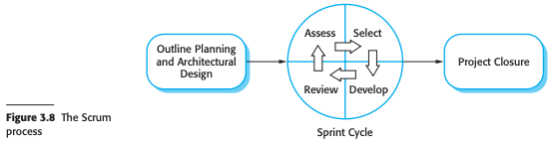
\includegraphics[width=8cm]{./graphics/scrum.png}
	\caption{A diagram of the scrum methodology	\cite{sommerville_2018}.}
	\label{fig:scrum}
	
\end{figure}
        
        The inspiration for this methodology was that an agile approach is widely used in industry and would be the most realistic for a project of this nature.  As only one person developed the application, the regular stand-up meetings and sprint reviews could not occur in the usual way.  A sprint review still took place at the end of every sprint, but no stand-up took place.  To keep track of tasks in the backlog and the current sprint, Trello was used, along with a third-party extension called TeamGantt.
        
        \begin{figure}[H]

	\centering
	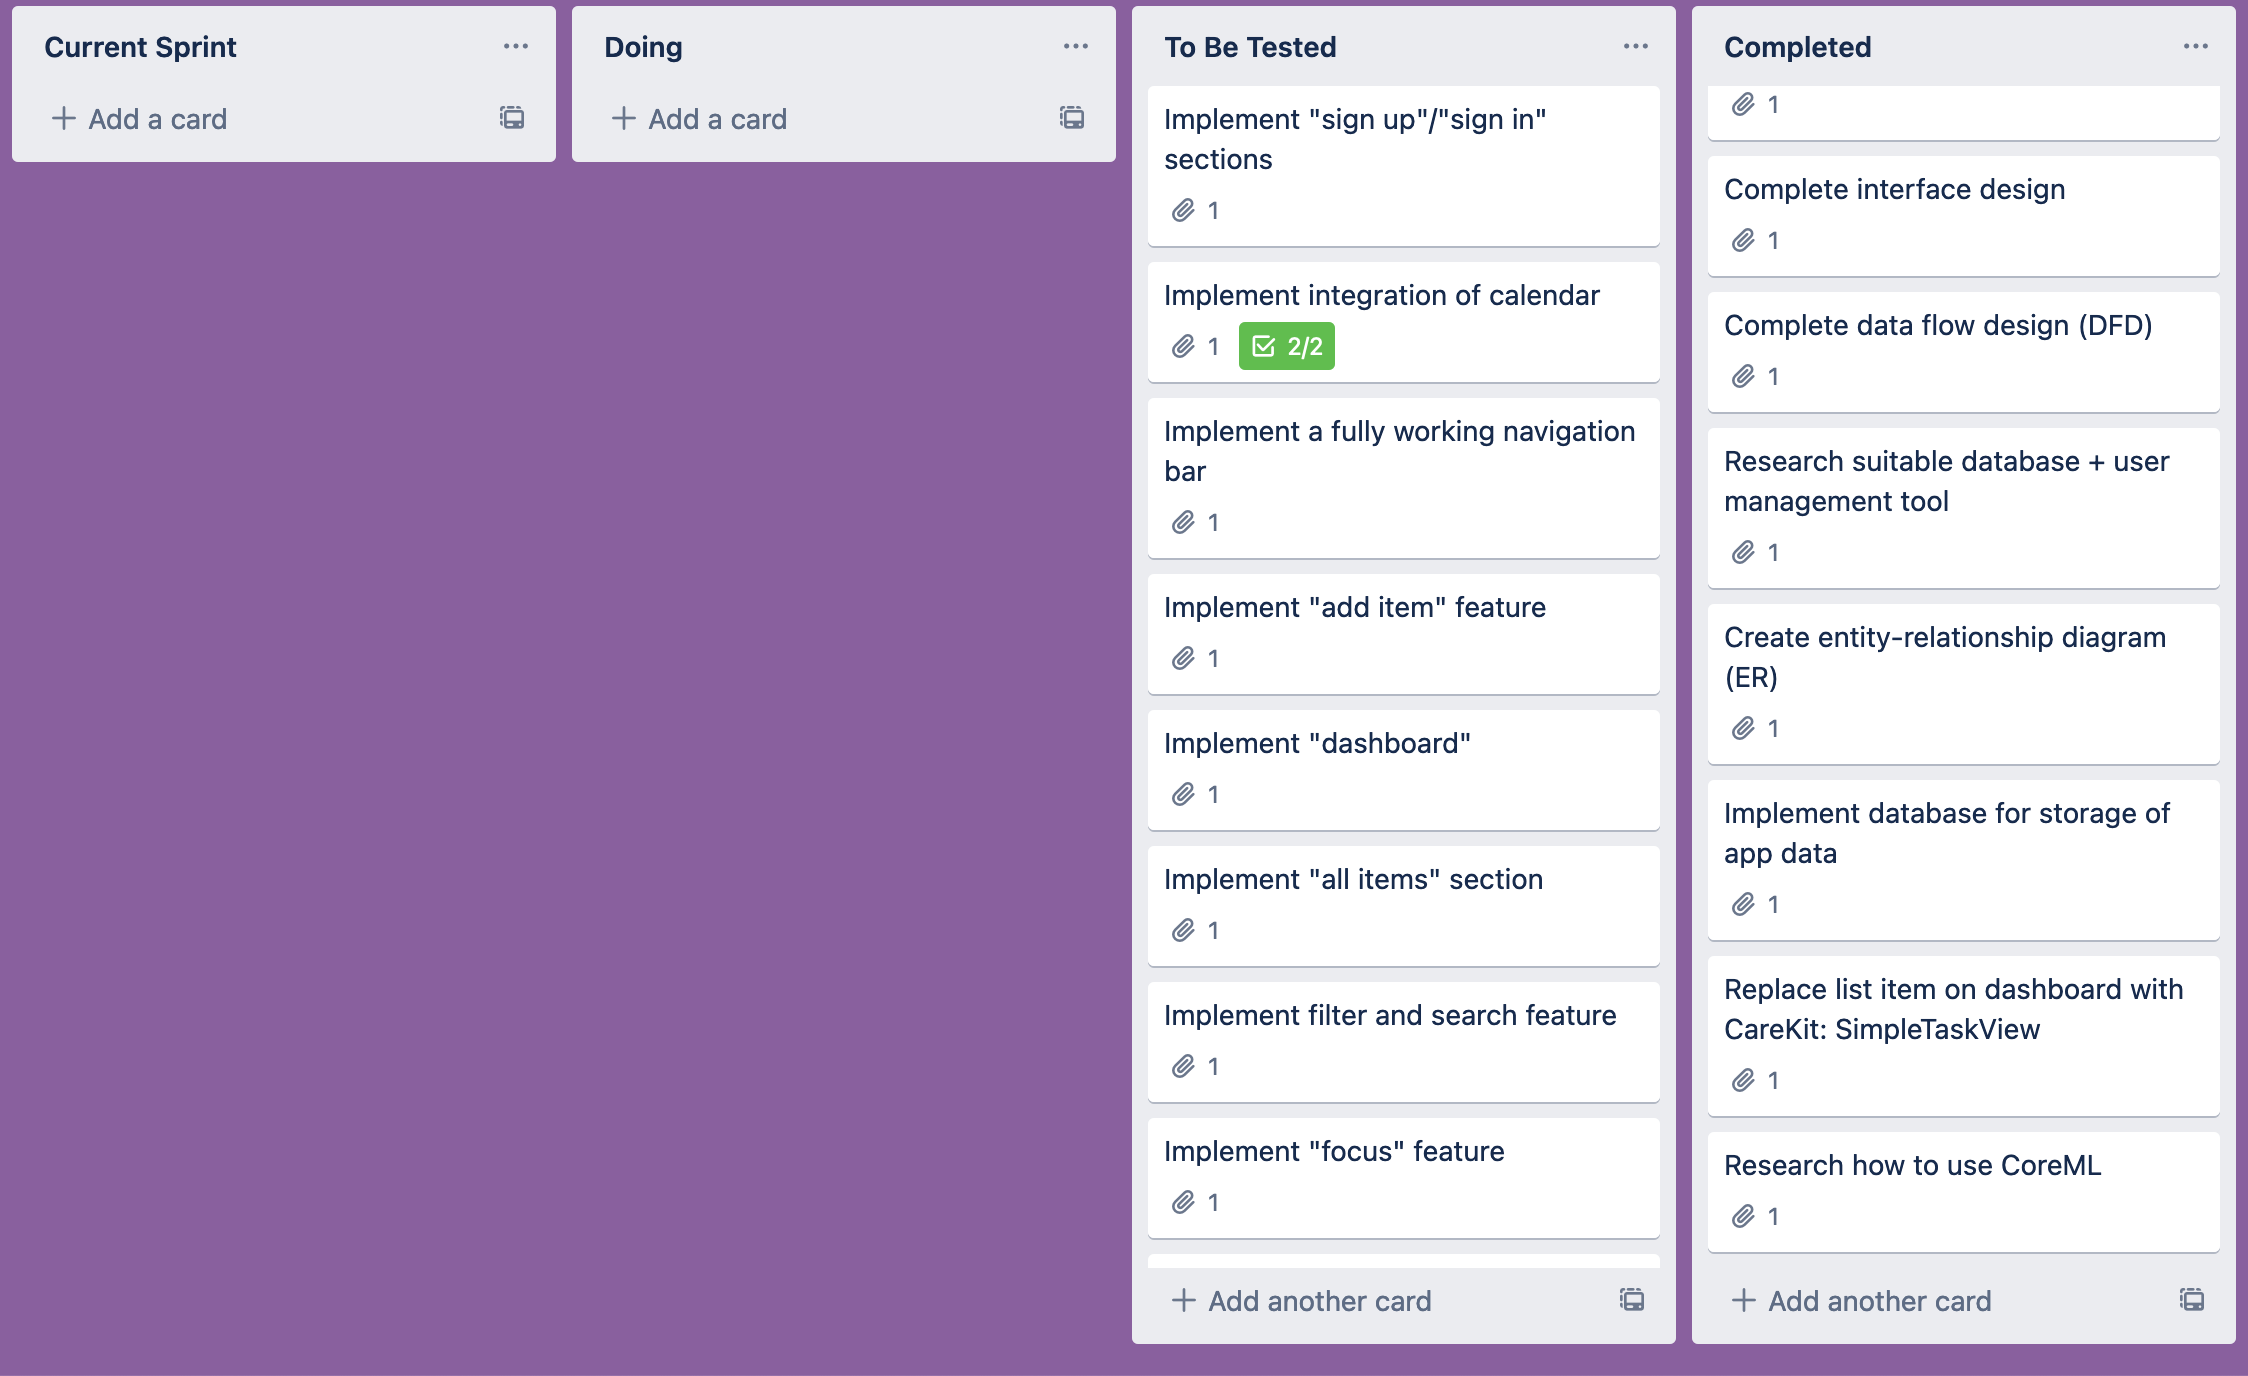
\includegraphics[width=12cm]{./graphics/trello.png}
	\caption{An image of Trello with completed tasks.}
	\label{fig:trello}
	
\end{figure}
        
        After using this model for the project, it seems to have remained the most suitable choice.  The regular sprint reviews ensured that the project stayed on track and completed tasks on time.  However, the prediction of upcoming tasks created before beginning the application could have been improved.  While implementing the application, it became clear some tasks that had not been anticipated were missing. These needed to be added in, resulting in the expected time frame of project completion being affected.  Overall, this did not affect the project's outcome, and the application mainly was completed on time apart from the testing phase (which will be discussed later in this document).
        
        For reference, the Gantt chart created before starting the application implementation has been placed in the appendix.
        
    \section{Risk analysis}
        \label{sec:sdl_risks}
        At the beginning of the project, potential risks had been defined and scored based on the likelihood and impact they would have on the project\cite{intial_document_pike} - Table~\ref{app::risk_table} in the appendix details these risks and their mitigation definitions.
        
        In Chapter~\ref{sec:reflection_risk}, a reflection of the risks specified at the beginning of the project will be discussed and any unforeseen risks that arose during the project and how they were dealt with.
